\newpage
\section{Reifegrad Methoden}

\subsection{Process Enterprise Maturity Model}


\subsection{SPICE}


\subsection{Business Process Maturity Model}

Das \ac{bpmm} ist ein Reifegradmodell, dass durch das herstellerunabhängige Industriekonsortium \ac{omg} entwickelt worden ist.
Die 1989 gegründete OMG umfasst über 800 Mitglieder von Unternehmen, wie z.B. Microsoft, Apple und IBM, die sich um die Entwicklung von Standards in der IT-Branche befassen.\par
Bekannte internationale Standards sind zum Beispiel die Unified Modeling Language zur Modellierung und Dokumentation von objektorientierten Systemen
und die grafische Geschäftsprozessmodellierung mit Business Process Modeling Notation. Der Reifegrad wird in fünf Stufen unterteilt, die in der 482 Seiten langen Veröffentlichung von OMG detailliert beschrieben werden.

\subsubsection{Reifegradstufen im \acs{bpmm}}

\begin{figure}[H]
  \centering
  \caption{\acs{bpmm}-Reifegradstufen}
  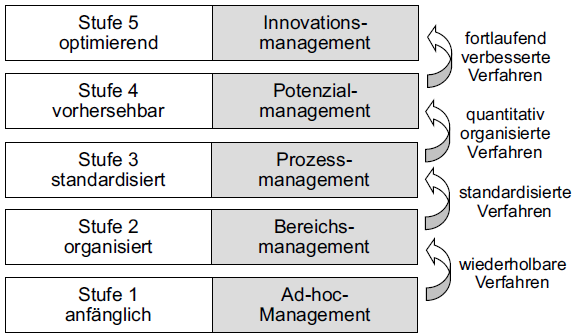
\includegraphics[width=12cm]{bpmmreifegradstufen.png}
  %\caption*{\footnotesize{\textbf{Quelle:} \cite[,2019,o.S.]{Capgemini2019}}}
  \label{fig:reifegradstufen}
\end{figure}

Bei \acs{bpmm} werden die Reifegrade in fünf Stufen unterteilt, siehe \autoref{fig:reifegradstufen}. Die \acs{omg} spricht hierbei von „maturity levels“ die aufeinander aufbauen. Ist eine Stufe erreicht, so gelten die vorherigen Voraussetzungen zum Erreichen dieser Reifegradstufe auch als erfüllt.
\textbf{Reifegradstufe 1 (initial)} ist ein Unternehmen, bei denen die Prozesse unvorhersehbar ablaufen. Die Unternehmensführung betreibt Ad-hoc-Management, bei dem nur bei konkret vorliegenden Problemen in Prozesse eingegriffen wird. Die Prozessqualität wird maßgeblich durch die Kompetenz der Mitarbeiter bestimmt. Maßnahmen zu einer kontinuierlichen Prozessverbesserung fehlen vollständig.
\par
\textbf{Reifegradstufe 2 (managed)} trifft zu, wenn auf Bereichs- beziehungsweise Abteilungsebene eine Management-Funktion zur Stabilisierung der Prozesse vorhanden ist. Die gelten jedoch nur für einen Bereich. Die Zusammenlegung von Bereichsübergreifenden (ähnlichen) Prozessen findet noch nicht statt und kann zu unterschiedlich angewendeten Verfahren für ähnliche Prozesse führen. Die Mitarbeiter arbeiten bereits mit wiederholbaren Prozessen, die lokal und operativ überwacht werden.
\par
\textbf{Reifegradstufe 3 (standardized)} besitzt erstmals Bereichsübergreifende Prozesse. Die Geschäftsprozesse sind standardisiert und erleichtern die Produkterstellung. Prozessverbesserungen werden bereits vorgenommen. Ein Prozessmanagement hält schriftlich erstmals bestimmte Verfahrensregeln fest und definiert Qualitätskriterien, die sich mit betriebswirtschaftlichen Kennzahlen messen lassen. Diese Kennzahlen und Kriterien sind eine erste Maßnahme zur Verbesserung einer Gesamtunternehmensplanung.
\par
\textbf{Reifegradstufe 4 (predictable)} setzt auf statistische Verfahren zur Messung von Prozessqualität. Die Ergebnisse aus Prozessen werden damit nicht nur planbar, sondern auch vorhersehbar. Ein Potenzialmanagement bewertet und überwacht die Arbeitsabläufe, um Verfahrensvarianten erkennen, verstehen und kontrollieren zu können. Erfahrungen aus der Anwendung von Standardprozessen werden mit den Arbeitseinheiten geteilt, damit weitere Prozessoptimierungen vorgenommen werden.
\par
\textbf{Reifegradstufe 5 (innovating)} beschreibt eine Organisation, dessen Geschäftsprozesse optimiert sind und kontinuierlich verbessert werden. Ein Innovationsmanagement sorgt organisationsübergreifend für systematische Prozessverbesserungen, die durch ein Change-Management umgesetzt werden.
\par

Details zu den einzelnen Stunfen können in nachfolgender \autoref{fig:bpmmreifegrade} angesehen werden.

\begin{figure}[H]
  \centering
  \caption{Details der Reifegradstufen im \acs{bpmm}}
  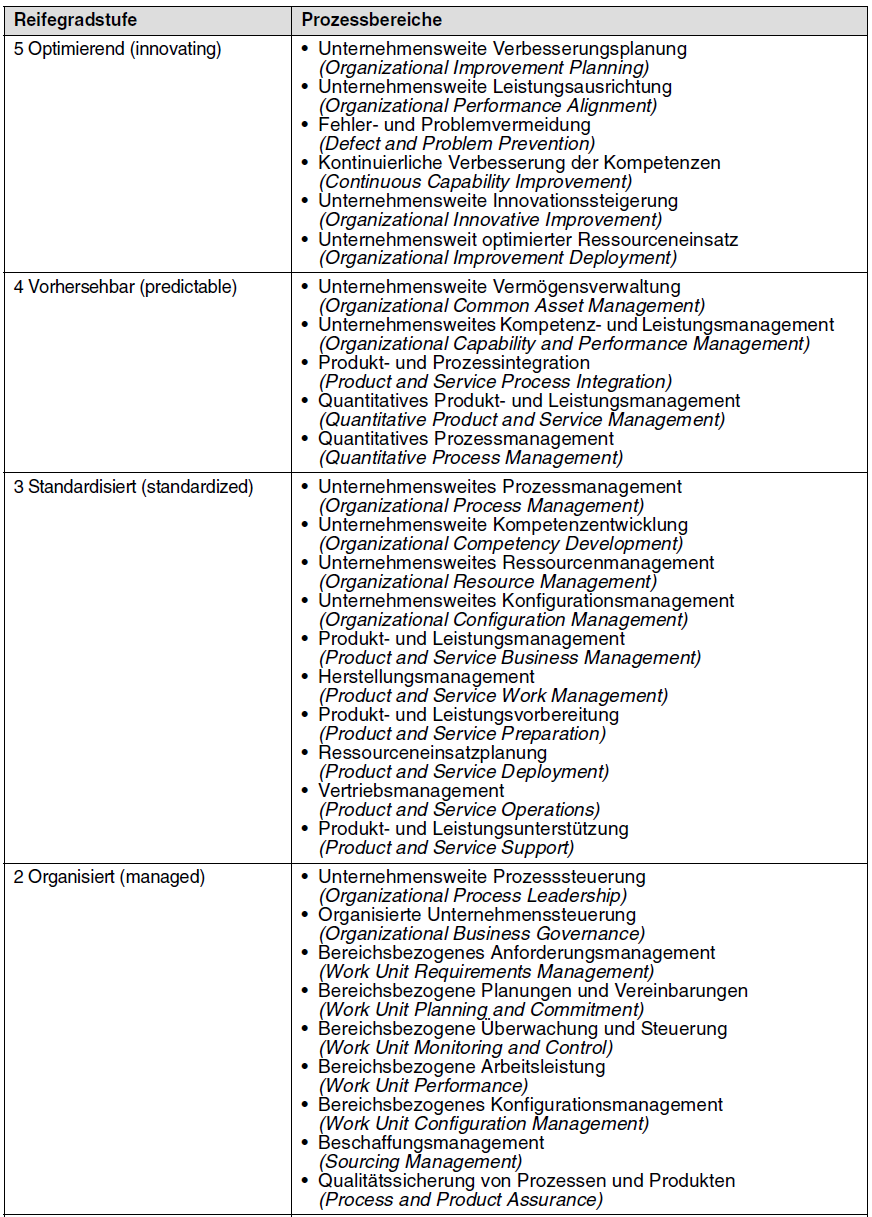
\includegraphics[width=12cm]{bpmmreifegrade.png}
  %\caption*{\footnotesize{\textbf{Quelle:} \cite[,2019,o.S.]{Capgemini2019}}}
  \label{fig:bpmmreifegrade}
\end{figure}

\subsubsection{Prozessbereiche und Zielesystematik}

Zur Ermittlung ob ein Reifegrad erreicht wurde müssen die Anforderungen der Prozessbereiche erfüllt werden. Jeder Reifegrad besteht aus fünf bis zehn Prozessbereichen. Jeder Prozessbereich wird wiederum in Ziele und Teilaktivitäten gegliedert. Die Teilaktivitäten sind die konkreten Anforderungsbeschreibungen, ohne explizit eine anzuwendende Methode anzugeben. Dadurch können Prozessbereiche auch durch bereits vorhandene Methoden erfüllt sein.

\subsubsection{Verantwortlichkeiten}

Damit die definierten Ziele der Prozessbereiche umgesetzt werden, werden diese bestimmten Unternehmensbereichen zugeteilt. \acs{bpmm} unterscheidet in die vier Unternehmensbereiche „Unternehmensleitung“, „mittleres Management“, „Querschnittsbereiche“ und „Ausführungsebene“. Eine Übersicht dieser Zuteilung und die jeweilige Reifegradstufe pro Prozessbereich sind in der nachfolgenden \autoref{fig:verantwortlichkeiten} ersichtlich.

\begin{figure}[H]
  \centering
  \caption{\acs{bpmm} Verantwortlichkeiten}
  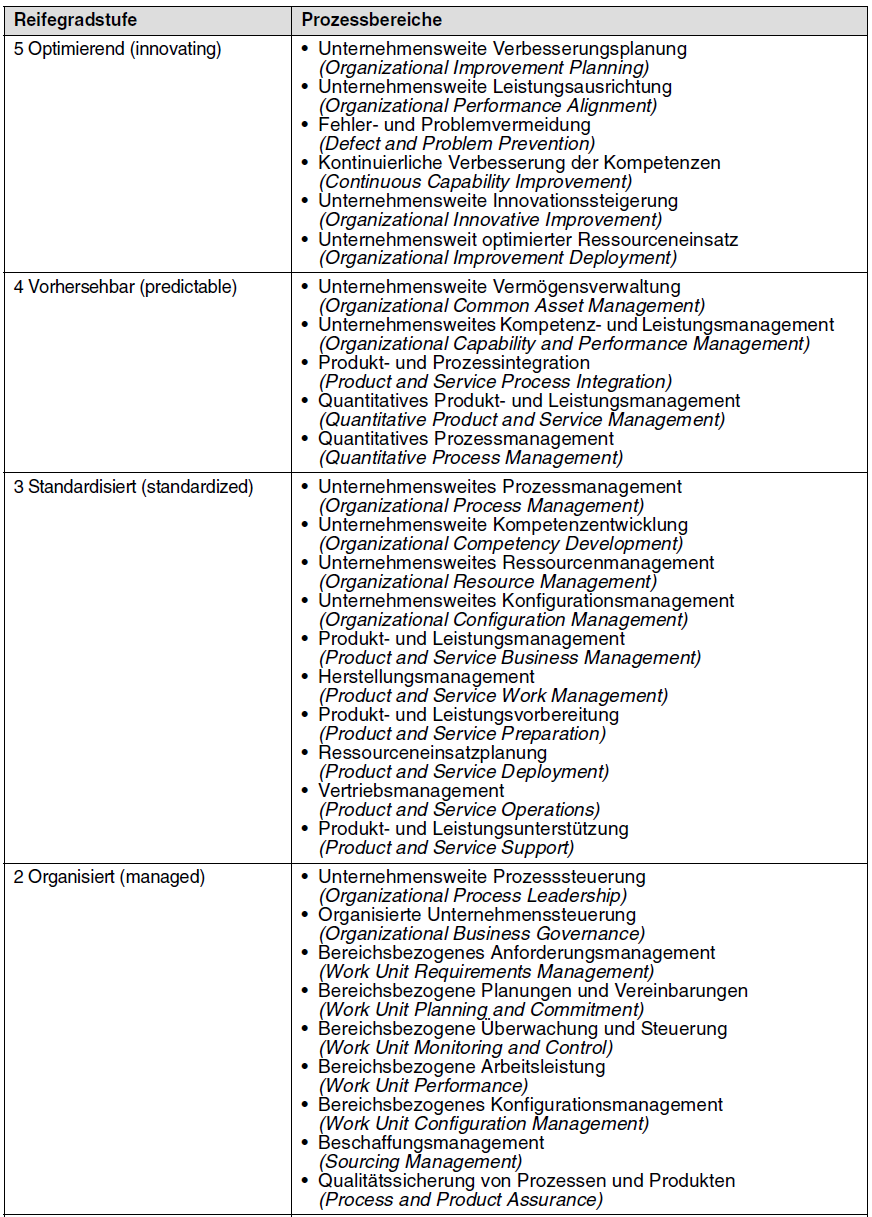
\includegraphics[width=12cm]{bpmmreifegrade.png}
  %\caption*{\footnotesize{\textbf{Quelle:} \cite[,2019,o.S.]{Capgemini2019}}}
  \label{fig:verantwortlichkeiten}
\end{figure}

Die Unternehmensleitung übernimmt dabei die unternehmensweiten Prozess- und Produktmanagement Aufgaben. Wichtige Ziele sind die kontinuierliche Verbesserung von Prozessen und der optimale Ressourceneinsatz. \par
Das mittlere Management kümmert sich um das bereichsbezogene Aufgabenmanagement. Dabei werden innerhalb der durch die Unternehmensleitung vorgegeben Handlungsrahmen quantitative Ziele umgesetzt. Auch die Überwachung und Steuerung des Bereichs fallen zu den Verantwortlichkeiten des mittleren Managements.\par
Die Querschnittsbereiche (Steuerungs- und Revisionseinheiten) unterstützen die Maßnahmen durch die genaue Dokumentation vorhandener Prozesse, um daraus Verbesserungspotenziale ableiten zu können. Es werden Stärken und Schwächen der Prozesse identifiziert. \par
Die Ausführungsebene besteht aus den Arbeitseinheiten und damit der unmittelbaren Wertschöpfungsquelle. Hier werden die Prozessverbesserungen operativ umgesetzt und quantitatives Prozessmanagement betrieben.

\subsubsection{Einsatzmöglichkeiten}

Das \acs{bpmm} lässt sich grundsätzlich in allen Branchen nutzen. Der Einsatz erfolgt durch konkrete und individuell festgelegte Methoden des Unternehmens, da \acs{bpmm} nur detaillierte Anforderungen und keine Methoden vorgibt.\par
Problematisch sehen Hogrebe und Nüttgens die eindeutige Zuordnung von Prozessbereichen zu Verantwortungsebenen, bei denen keine Verantwortlichkeiten zu unternehmensübergreifenden Prozessen im \acs{bpmm} definiert sind. Ein weiterer Punkt ist der Fokus auf ausschließliche Optimierung der Geschäftsprozesse ohne Angleichung der Aufbau- und Ablauforganisation.\par
Mit \acs{bpmm} werden die detailliert formulierten Anforderungen im Unternehmen dauerhaft verankert und erzeugt eine Unternehmenskultur, die eine stetige Prozessverbesserung in allen Bereichen anstrebt. \acs{bpmm} bietet alternativ auch die Möglichkeit, nur teilweise in bestimmten Bereichen angewendet zu werden.\par
Abschließend nennen Hogrebe und Nüttgens das \acs{bpmm} ein klar strukturiertes Reifegradmodell mit einer hohen Detailtiefe bei der Beschreibung erforderlicher Schritte zur Erreichung von Reifegradstufen. Der Einsatz von \acs{bpmm} sollte jedoch von der Geschäftsleitung wohlüberlegt sein, da dies zu einem Eingriff in die Organisationsstruktur führt und Ressourcen bindet.
